\documentclass[compress,red]{beamer}
\mode<presentation>

\usetheme{Warsaw}

% define your own colors:
\definecolor{Red}{rgb}{1,0,0}
\definecolor{Blue}{rgb}{0,0,1}
\definecolor{Green}{rgb}{0,1,0}
\definecolor{magenta}{rgb}{1,0,.6}
\definecolor{lightblue}{rgb}{0,.5,1}
\definecolor{lightpurple}{rgb}{.6,.4,1}
\definecolor{gold}{rgb}{.6,.5,0}
\definecolor{orange}{rgb}{1,0.4,0}
\definecolor{hotpink}{rgb}{1,0,0.5}
\definecolor{newcolor2}{rgb}{.5,.3,.5}
\definecolor{newcolor}{rgb}{0,.3,1}
\definecolor{newcolor3}{rgb}{1,0,.35}
\definecolor{darkgreen1}{rgb}{0, .35, 0}
\definecolor{darkgreen}{rgb}{0, .6, 0}
\definecolor{darkred}{rgb}{.75,0,0}

\xdefinecolor{olive}{cmyk}{0.64,0,0.95,0.4}
\xdefinecolor{purpleish}{cmyk}{0.75,0.75,0,0}

\useoutertheme[subsection=false]{smoothbars}

% include packages
\usepackage{kotex}
\usepackage{subfigure}
\usepackage{multicol}
\usepackage{amsmath}
\usepackage{epsfig}
\usepackage{graphicx}
\usepackage[all,knot]{xy}
\usepackage{url}
\usepackage{multimedia}
\usepackage{hyperref}
\usepackage{setspace}


\title{\textbf{\LaTeX}}
\subtitle{Beamer example}
\author{Aejin Ju}
\institute{Department of Information and Statistics}
\date{August 11, 2018}


\begin{document}

\frame{
	\titlepage
}

\section[Outline]{}
\frame{\tableofcontents}


\section{LaTeX의 특징}
\frame{
\frametitle{LaTeX의 특징}

\begin{itemize}

	\item 공백 : 공백문자(whitespace), 즉 빈 칸(blank), 탭(tab) 등은 
				\LaTeX에서 모두 동일하게 "스페이스" 로 처리함

	\vspace{0.25cm} \pause

	\item 특수문자 : \#, \$, \%, \^{}, \&, \_, \{, \}, \~{}, $\setminus$는 
					\LaTeX에서 특별한 의미를 갖거나 어떤 글꼴로도 나타낼 수 없음

	\vspace{0.25cm} \pause

	\item \LaTeX 명령 : 백슬래시 $\setminus$로 시작하여 문자(letter)만으로 
						이루어진 이름을 갖고 대소문자를 구분함

	\vspace{0.25cm} \pause

	\item 주석 : \% 문자를 만나면 그 줄(행)의 나머지 부분과 줄바꿈을 무시함

\end{itemize}
}


\section{Math}

\subsection{벡터의 p-norm}
\frame{
\frametitle{벡터의 p-norm}

	\begin{block}{\footnotesize벡터의 p-norm}
		\scriptsize 벡터 $\textbf{X}=(x_1, x_2, \cdots, x_n)$의 크기 : \vspace{-0.3cm}
			\center{$\Vert \textbf{X} \Vert_{p} = \left( |x_1|^p + |x_2|^p + \cdots +|x_n|^p
			 \right)^{\frac{1}{p}}$}  \\ \vspace{0.2cm}
	\end{block} \vspace{0.2cm} 
	
	\begin{block}{\footnotesize 벡터 $\textbf{X}$과 $\textbf{Y}$의 차이의 크기}
		\scriptsize 벡터 $\textbf{X}=(x_1, x_2, \cdots, x_n)$, 
				벡터 $\textbf{Y}=(y_1, y_2, \cdots, y_n)$\vspace{-0.1cm}
		\center {$\Vert \textbf{X} - \textbf{Y} \Vert_{p}
				= \left[ \displaystyle \sum_{i=1}^{n} 
				| x_i - y_i |^{p} \right] ^{\frac{1}{p}}$} \vspace{0.2cm}
	\end{block}
	
	\begin{itemize}
		\footnotesize
		\item $uniform$ $norm$ : $\Vert \textbf{X} - \textbf{Y} \Vert_{\infty}
				= max_{1 \le i \le n} |x_{i} - y_{i}|$	\vspace{0.2cm}
		\item $1-norm$ : $\Vert \textbf{X} - \textbf{Y} \Vert_{1}
				= \sum_{i=1}^{n} |x_{i} - y_{i}|$ \vspace{0.1cm}
		\item $2-norm$ : $\Vert \textbf{X} - \textbf{Y} \Vert_{2}
				= \left[ \sum_{i=1}^{n} |x_{i} - y_{i}|^{2} \right]^\frac{1}{2}$ \vspace{0.5cm} 
	\end{itemize}	
}

\subsection{함수의 p-norm}
\frame{
\frametitle{함수의 p-norm}

	\begin{block}{\footnotesize 함수의 p-norm}
		\scriptsize 
		$D$는 $f(x)$가 정의된 영역이다. \\  \vspace{-0.3cm}
 		\center{$\Vert f(x) \Vert_{p} =
		\left[ \int_{D}^{} |f(x)|^p dx \right] ^{\frac{1}{p}}$ } \vspace{0.2cm}
	\end{block} \vspace{0.2cm} 
	
	\begin{block}{\footnotesize함수 $f(x)$와 $g(x)$의 차이의 크기}
		\scriptsize 
		$D$는 $f(x)$와 $g(x)$가 정의된 영역이다. \\ \vspace{-0.3cm}
 		\center{$\Vert f(x)-g(x) \Vert_{p} =
		\left[ \int_{D}^{} |f(x)-g(x)|^p dx \right] ^{\frac{1}{p}}$ } \vspace{0.2cm} 
	\end{block}
	
	\begin{itemize}
		\footnotesize
		\item $uniform$ $norm$ : ${\Vert f(x)-g(x) \Vert}_{\infty} =
				max_{x \in D} |f(x)-g(x)|$  	\vspace{0.2cm}
		\item $1-norm$ : $\Vert f(x)-g(x) \Vert_{1} = \int_{D} | f(x) - g(x) | dx$ \vspace{0.1cm}
		\item $2-norm$ : ${\Vert f(x)-g(x) \Vert}_{2} =
				\left[ \int_{D} | f(x) - g(x) |^{2} dx \right] ^{\frac{1}{2}} $ \vspace{0.5cm} 
	\end{itemize}
}


\section{Tables}
\subsection{Discrete Distributions}
\frame{
\frametitle{Discrete Distributions}

	\begin{table}[h!] \scriptsize
		\begin{center}			
			\begin{tabular}{ c | c } 
				\hline
				Distribution & Probability Function \\
				\hline 
				\textbf{binomial} 
				& $ \displaystyle p(y) = \binom{n}{y} p^{y} (1-p)^{n-y} $ \\ 
				\hline
				\textbf{geometric} 
				& $ \displaystyle p(y) = \frac{\binom{r}{y} \binom{N-r}{n-y}}{\binom{N}{n}} $ \\
				\hline
				\textbf{hypergeometric} 
				& $ \displaystyle p(y) = \frac{\binom{r}{y} \binom{N-r}{n-y}}{\binom{N}{n}} $ \\
				\hline
				\textbf{poisson} 
				& $ \displaystyle p(y) = \frac{\lambda^{y} e^{-\lambda}}{y!} $ \\
				\hline
				\textbf{negative binomial} 
				& $ \displaystyle p(y) = \binom{y-1}{r-1} p^{y} (1-p)^{y-r} $ \\
				\hline
			\end{tabular}		
		\end{center}
	\end{table}	
}



\subsection{Continuous Distributions}
\frame{
\frametitle{Continuous Distributions}

	\begin{table}[h!] \scriptsize
		\begin{center}			
			\begin{tabular}{ c | c } 
				\hline
				Distribution & Probability Function \\
				\hline 
				\textbf{uniform} 
				& $ \displaystyle f(y) = \frac{1}{\theta_{2} - \theta_{1}} $ \\
				\hline
				\textbf{normal} 
				& $ \displaystyle f(y) = \frac{1}{\sigma \sqrt{2\pi}}
				\exp \left[ - \left( \frac{1}{2\sigma^{2}} \right) 
				(y-\mu)^{2} \right] $ \\
				\hline
				\textbf{exponential} 
				& $ \displaystyle f(y) = \frac{1}{\beta} e^{-y/\beta}, \beta>0 $ \\
				\hline
				\textbf{gamma} 
				& $ \displaystyle f(y) = \left[ \frac{1}{\Gamma(\alpha) \beta^{\alpha}} \right]
				y^{\alpha - 1} e^{-y/\beta} $ \\
				\hline
				\textbf{chi-square} 
				& $ \displaystyle f(\chi^{2}) = 
				\frac{(\chi^2)^{(\nu/2)-1} e^{-\chi^{2}/2}}
				{2^{\nu/2} \Gamma (\nu/2) }  $ \\
				\hline
				\textbf{beta} 
				& $ \displaystyle f(y) = \left[ 
				\frac{\Gamma(\alpha + \beta)}{\Gamma(\alpha) \Gamma(\beta)} \right]
				y^{\alpha - 1} (1-y)^{\beta - 1} $ \\
				\hline
			\end{tabular}		
		\end{center}
	\end{table}
}


\section{Figures}
\frame{
\frametitle{Figures}

	\begin{columns} \footnotesize
		\begin{column}{0.5\textwidth}
			\begin{itemize}
				\item binomial distribution
			\end{itemize}
			\begin{figure}
				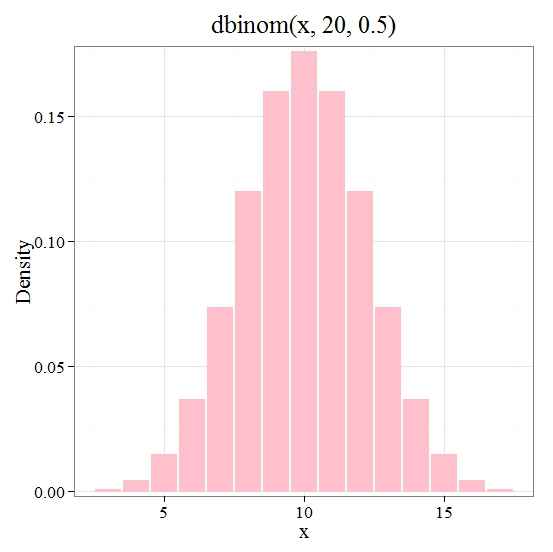
\includegraphics[width=0.9\textwidth]{binomial_distribution.jpeg}
			\end{figure} \scriptsize
			\center{$\displaystyle p(y) = \binom{n}{y} p^{y} (1-p)^{n-y} $} 
		\end{column}
		
		\begin{column}{0.5\textwidth}
			\begin{itemize}
				\item uniform distribution
			\end{itemize}
			\begin{figure}
				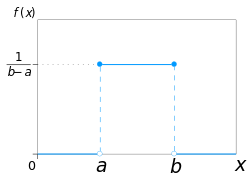
\includegraphics[width=0.9\textwidth]{uniform_distribution.png}
			\end{figure}
			\center{$ \displaystyle f(y) = \frac{1}{\theta_{2} - \theta_{1}} $} 
		\end{column}
	\end{columns}	
}


\end{document} 